\textbf{Para el mundo de un robot de servicio de cafetería, enuncia: sus sensores, sus efectores, su ambiente, su entorno de trabajo. Además, propón una medida de rendimiento para que su agencia sea racional. Además, indica qué tipo de agente sería mejor implementar para su servicio: basado en modelo, que aprende, dirigido por tabla, o reactivo simple (1 pt.).} \vspace{.3cm}

Primero que nada, estoy considerando un bot como este:

\begin{figure}[H]
    \centering
    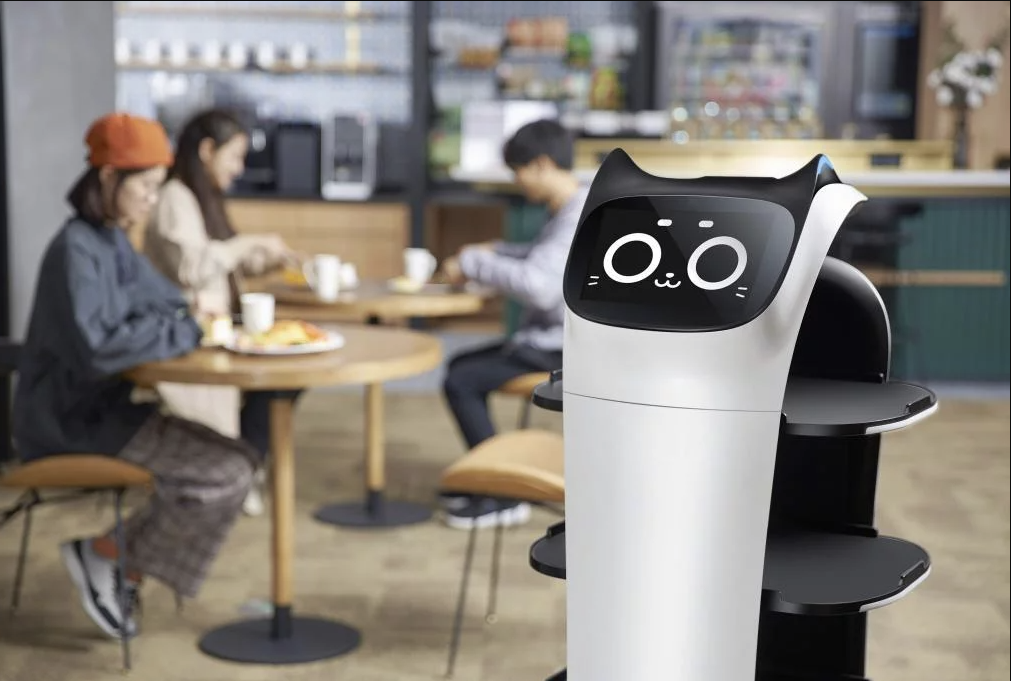
\includegraphics[width=10cm]{src/Img/robot.png}
    \caption{\cite{seboticsImagen}}
\end{figure}

\begin{itemize}
    \item \textbf{Entorno de trabajo:}  
    Voy a comenzar describiendo el tipo de ambiente según las clasificaciones (véase pregunta 9). El ambiente es parcialmente observable, se espera que haya varios agentes interactuando de manera cooperativa, por lo que es un entorno estocástico y muy cambiante. Creo que sería más sencillo tratarlo de manera episódica, con episodios de mayor duración. Además, el entorno es dinámico y se desarrolla de forma continua.
    \begin{itemize}
        \item \textbf{Sensores:}  
        Como mínimo, el robot necesitará cámaras (al menos 3), un velocímetro, algún tipo de pantalla, micrófonos y, quizás, GPS.
        \item \textbf{Efectores:}  
        En este modelo, contará con ruedas, motor, freno, bocina, pantalla y acelerador. No requiere un mecanismo para agarrar el contenido, ya que éste se coloca en sus repisas.
        \item \textbf{Ambiente:}  
        Se trata de una cafetería, con numerosos elementos móviles como sillas, mesas y personas, y algunos elementos estáticos como paredes o estantes.
        \item \textbf{Medida de rendimiento:}  
        Una buena medida de rendimiento podría incluir la rapidez en el servicio, la seguridad en la manipulación de las bebidas, la maximización de ganancias, la reducción de colisiones, el rendimiento de la batería y la satisfacción de los clientes (evaluada mediante encuestas rápidas).
    \end{itemize}
    
    \item \textbf{Tipo de agente:}  
    Considero que el agente debe ser capaz de aprender, ya que sus interacciones con el entorno son complejas. Dado que se enfrenta a un ambiente tan cambiante y con múltiples objetivos, es necesario que sea adaptable. Por ello, se recomienda implementar un agente basado en utilidad, que integre un modelo para poder distinguir lo que está percibiendo y determinar la trayectoria óptima.
\end{itemize}
